

\subsection{Соединения азота, способы получения, химическое поведение, электронное и геометрическое строение молекул.}

\subsubsection*{Азот}

\textbf{Способы получения}

1) Промышленный

Фракционирование воздуха или разделение воздуха на мембранах

2) Лабораторный

$$2NaN_3 \rightarrow 2Na + 3N_2$$
$$NH_4NO_4 \rightarrow N_2 + H_2O$$
$$NH_3 + O_2 \rightarrow N_2 + H_2O$$

\textbf{Химические свойства}

Низкая реакционная способность

1) С Ме при нагревании ( с Li при н.у.)

$$3Mg + N_2 \rightarrow Mg_3N_2 (450^{\circ})$$
$$6Li + N_2 \rightarrow 2Li_3N$$

2) C $H_2$

$$N_2 + H_2 \leftrightarrows NH_3 (p,t,kat)$$

3) С $O_2$ (электрический разряд)

$$N_2 + O_2 \rightarrow 2NO$$

4) С комплексами переходных металлов

$$[Ru(NH_3)_5(H_2O)]Cl_3 + N_2 + Zn/Hg \rightarrow [Ru(NH_3)_5(N_2)]Cl_2 + ZnCl_2 + Hg + H_2O$$

\textbf{Электронное и геометрическое строение}

Линейная молекула, $\mu=0$\\
Строение молекулярное в паре, жидкости и твердой фазы\\
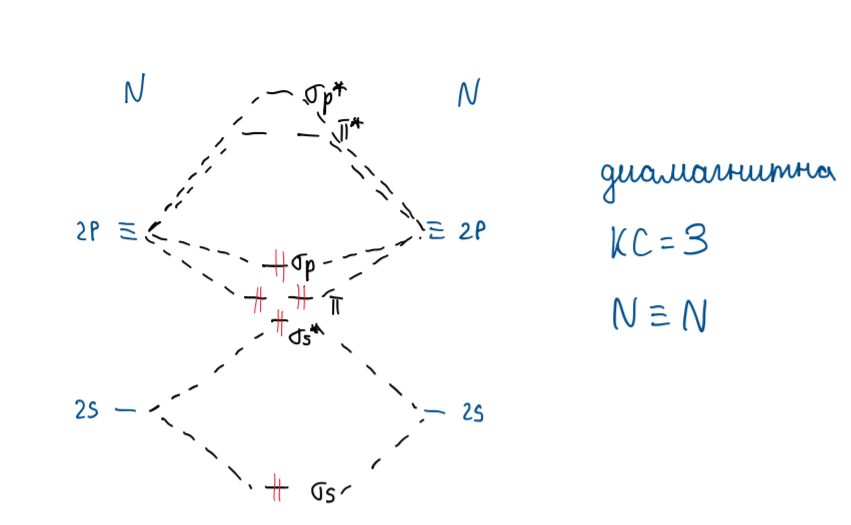
\includegraphics{images/8v1.png}

\subsubsection*{$NH_3$}

\textbf{Способы получения}

$$Mg_3N_2 + H_2O \xrightarrow{OH^-} NH_3 + Mg(OH)_2$$
$$NH_4Cl + Ca(OH)_2 \rightarrow CaCl_2 + H_2O + NH_3$$
$$KNO_3 + Zn + KOH + H_2O \rightarrow NH_3 + K_2[Zn(OH)_4]$$

Процесс Боша-Хабера:

$$ N_2 + H_2 \leftrightarrows NH_3 (p=200 atm, \ T = 450^{\circ},\ Fe_3O_4 + Al_2O_3 + K_2O + SiO_2)$$

\textbf{Химические свойства}

1) Автоионизация

$$NH_3 \leftrightarrows NH_4^+ + NH_2^-$$

2)  Основание

$$NH_3 + H_2O \leftrightarrows NH_4^+ + OH^-$$
$$NH_3 + HR \rightarrow NH_4R \ (R - kislotn. ost)$$

3) Окисление

$$NH_3 + O_2 \xrightarrow{Rh/Pt} NO + H_2O$$
$$NH_3 + O_2 \rightarrow N_2 + H_2O$$
$$NH_3 + O_2 \xrightarrow{Rh/Pt} NH_4NO_3 + H_2O$$

4) Жидкий аммиак растворяет щелочные металлы:

$$K \xrightarrow{NH_{3(liq.)}} K_{solv}^+ + e_{solv}^+$$
$$ K + Ge \xrightarrow[en]{NH_{3(liq.)}} K_4Ge_9\cdot en$$

Соли Цинтля - сильнейшие восстановители

$$NH_3 + K \rightarrow KNH_2 + H_2$$

5) Образование комплексных соединений с солями Cu и Ag

$$Cu(NO_3)_2 + NH_3 \rightarrow [Cu(NH_3)_4](NO_3)_2$$
$$AgNO_3 + NH_3 \rightarrow [Ah(NH_3)_2]NO_3$$

\textbf{Электронное и геометрическое строение}

Пирамидальная молекула, плоская форма не существует, но можно оценить с помощью квантово-химических расчетов.

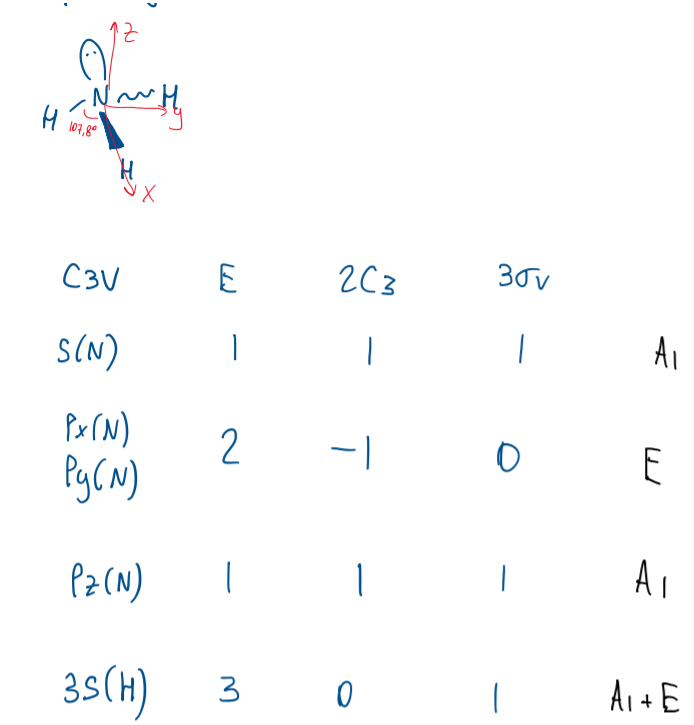
\includegraphics[scale=0.8]{images/8v2.png}

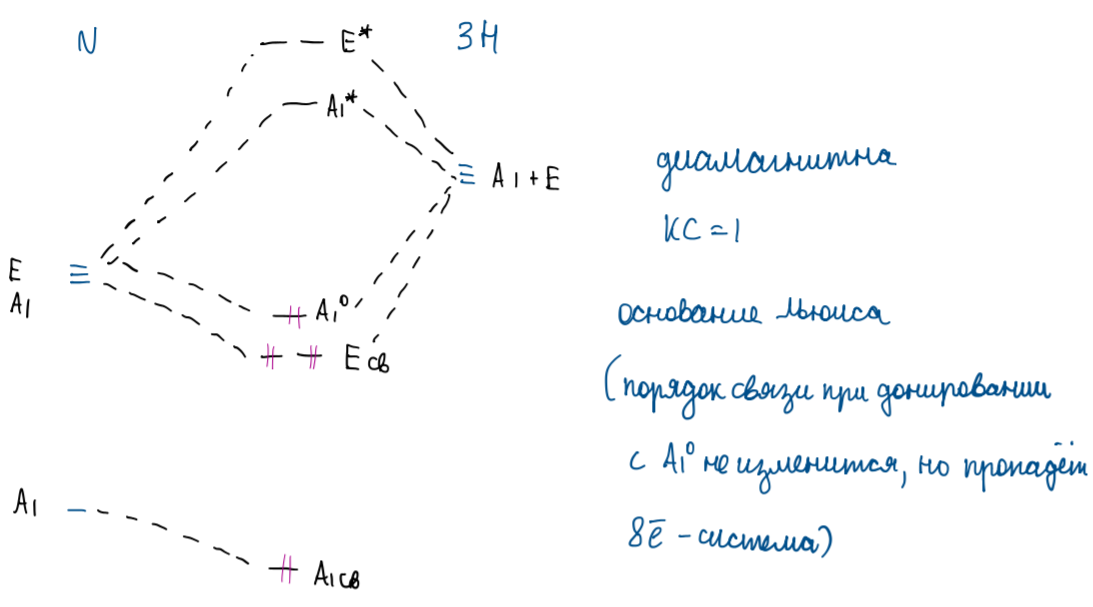
\includegraphics[scale=0.8]{images/8v3.png}

\subsubsection*{$N_2H_4$}

\textbf{Способы получения}

$$NaClO + NH_3 \xrightarrow{Mn^{2+}} NaCl + H_2O + N_2H_4$$

\textbf{Химические свойства}

1) Основание

$$N_2H_4 + H_2O \leftrightarrows N_2H_5^+ + OH^-$$
$$N_2H_5^+ + H_2O \leftrightarrows N_2H_6^{2+} + OH^-$$

2) Окисление

$$N_2H_4 + O_2 \rightarrow N_2\uparrow + H_2O \uparrow$$

3) Разложение

$$N_2H_4 \xrightarrow{200-300^{\circ}} N_2 + NH_3$$
$$N_2H_4 \xrightarrow{Pt/Rh/Pd} N_2 + H_2$$

4) Сильный восстановитель

$$N_2H_4 + Zn + HCl \rightarrow ZnCl_2 + NH_4Cl$$
$$KMnO_4 + N_2H_4 + H_2SO_4 \rightarrow K_2SO_4 + MnSO_4 + H_2O + N_2$$

\textbf{Электронное и геометрическое строение}

Две группы $NH_2$, повернутые относительно друг друга, молекула полярная.

У атомов азота по одной НЭМ.

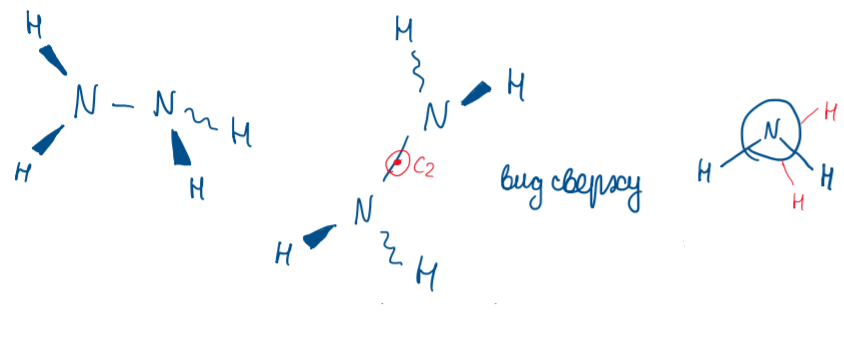
\includegraphics{images/8v4.png}

\subsubsection*{$HN_3$}

\textbf{Способы получения}

$$NaNH_2 + N_2O \xrightarrow{200^{\circ}} NaN_3 + NaOH + NH_3$$
$$NaN_3 + H_2SO_4 \rightarrow Na_2SO_4 + NH_3$$

\textbf{Химические свойства}

1) Слабая кислота

$$HN_3 \leftrightarrows H^+ + N_3^-$$

2) Окислитель

$$Cu + HN_3 \rightarrow Cu(N_3)_2 + N_2 + NH_3$$
$$HCl + HN_3 \rightarrow NH_4Cl + Cl_2 + N_2$$

3) Разложение

$$HN_3 + H_2O \rightarrow N_2 + NH_2OH$$

4) Соли - азиды, неустойчивы и взрывчаты

Азиды щелочных металлов (не Li) и тяжелых металло при t $\rightarrow Me + N_2$
(Получение очень чистых металлов)

Азиды щелочноземельных металлов и Li разлагаются на нитрид и $N_2$\\
\\

\textbf{Электронное и геометрическое строение}

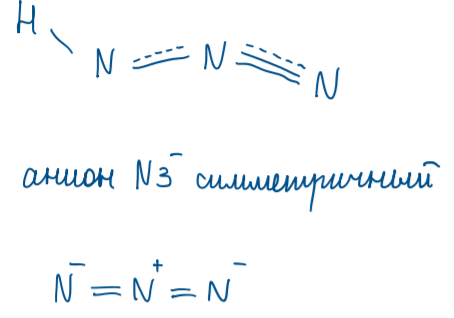
\includegraphics{images/8v5.png}

Можно рассмотреть как результат замены в $N_2O$ атома $O$ на группу $N-H$

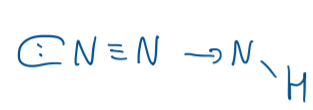
\includegraphics{images/8v6.png}

\subsubsection*{$N_2O$}

\textbf{Получение}

$$NH_4NO_3 \xrightarrow{250^{\circ}} N_2O + H_2O$$
$$NH_2OH + HNO_2 \rightarrow N_2O + H_2O$$

\textbf{Химические свойства}

1) Несолеобразующий

2) Разложение

$$N_2O \xrightarrow{700^{\circ}} N_2 +O_2$$

3) Поддерживает горение

$$N_2O + H_2 \rightarrow N_2 + H_2O$$
$$N_2O + C \rightarrow N_2 + CO$$
$$N_2O + P \rightarrow N_2 + P_2O_5$$

\textbf{Электронное и геометрическое строение}

Линейная молекула, помимо $\sigma$-связей есть второстепенное взаимодействие p-орбиталей 2-типа.

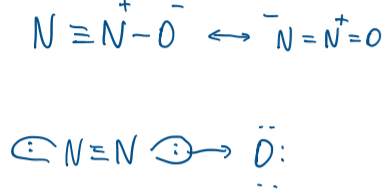
\includegraphics{images/8v7.png}

\subsubsection*{$NO$}

\textbf{Получение}

1) Каталитическое окисление аммиака (промышленный способ)

$$NH_3 + O_2 \xrightarrow{kat, 1000^{\circ}} NO + H_2O$$
$$N_2 + O_2 \xrightarrow{2000^{\circ}} NO$$

2) В лабаратории

$$ Cu + HNO_{3(razb.)}\rightarrow Cu(NO_3)_2 + H_2O + NO$$
$$KNO_2 + KI + H_2SO_4 \rightarrow K_2SO_4 + I_2 + NO$$

3) Легко окисляется $O_2$ и $Hal_2$

$$NO + O_2 \rightarrow NO_2$$
$$NO + Cl_2 \rightarrow NOCl$$

4) Нерастворим в воде, не реагирует с $H^+$ и $OH^-$

5) Слабый окислитель

$$NO + H_2 \rightarrow N_2 + H_2O$$
$$NO + SO_2 \rightarrow N_2 + SO_3$$

6) Слабый восстановитель

$$NO + K_2Cr_2O_7 + H_2SO_4 \rightarrow HNO_3 + K_2SO_4 + Cr_2(SO_4)_3 + H_2O$$

\textbf{Электронное и геометрическое строение}

Линейная молекула-радикал, нет димеризации

$$NO^- \xleftarrow{+e} NO \xrightarrow{-e}  NO^+$$

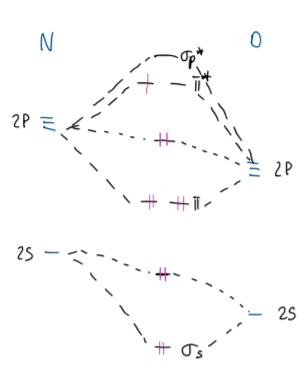
\includegraphics{images/8v8.png}

\subsubsection*{$N_2O_3$}

\textbf{Способы получения}

$$NO_2 + NO \leftrightarrows N_2O_3$$

\textbf{Химические свойства}

1) Неусточив разлагается на $NO$ и $NO_2$

2) Ангидрид азотистой кислоты $HNO_2 \Rightarrow$ все свойства кислотных оксидов

\textbf{Электронное и геометрическое строение}

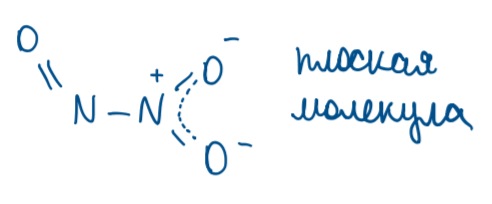
\includegraphics{images/8v9.png}

\subsubsection*{$NO_2$}

\textbf{Способы получения}

$$NO + O_2 \rightarrow Cu(NO_3)_2 + NO_2 + H_2O$$
$$Cu + HNO_{3(konc)} \rightarrow Cu(NO_3)_2 + NO_2 + H_2O$$

Разложение нитратов:

$$Cu(NO_3)_2 \rightarrow CuO + NO_2 + O_2$$

\textbf{Химические свойства}

1) С $H_2O$

$$NO_2 + H_2O \rightarrow HNO_2 + HNO_3$$
$$NO_2 + H_2O + O_2 \rightarrow HNO_3$$

2) С щелочами

$$NO_2 + NaOH \rightarrow NaNO_2 + NaNO_3 + H_2O$$

3) Окислитель

$$NO_2 + SO_2 \rightarrow NO + SO_3$$
$$NO_2 + C \rightarrow CO_2 + N_2$$
$$NO_2 + P \rightarrow P_2O_5 + NO$$

4) Димеризация

$$2NO_2 \leftrightarrows N_2O_4$$

\textbf{Электронное и геометрическое строение}

У $NO_2$ 1 неспаренный электрон на связывающей орбитали $\Rightarrow$ выгодна димеризация

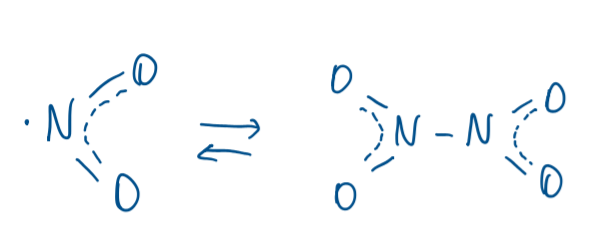
\includegraphics{images/8v10.png}

\subsubsection*{$N_2O_5$}

\textbf{Способы получения}

$$NO_2 +O_3 \rightarrow N_2O_5 + O_2$$
$$HNO_3  + P_2O_5 \rightarrow HPO_3 + N_2O_5$$

\textbf{Химические свойства}

1) Ангидрит азотной кислоты $HNO_3 \Rightarrow$ все свойства кислотных оксидов

2) Сильный окислитель

$$N_2O_5 + I_2 \rightarrow I_2O_5 + N_2$$

3) Легко разлагается ( при нагревании со взрывом)

$$N_2O_5 \rightarrow NO_2 + O_2$$

\textbf{Электронное и геометрическое строение}

Не все атомы в одной плоскости

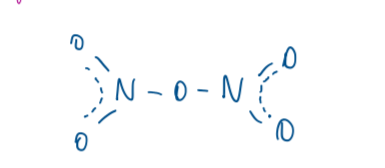
\includegraphics{images/8v11.png}

\subsubsection*{$H_2N_2O_2$ - азотноватистая кислота}

\textbf{Способы получения}

$$Ag_2N_2O_2 + HCl \xrightarrow[-AgCl]{efir} H_2N_2O_2$$

\textbf{Химические свойства}

1) Слабая неустойчивая кислота

$$H_2N_2O_2 \xrightarrow{t} N_2O \uparrow + H_2O$$

2) Горение

$$H_2N_2O_2 +O_2 \rightarrow HNO_2 + HNO_3$$

3) Образует комплексы в d-металлами

\textbf{Электронное и геометрическое строение}

Плоская молекула

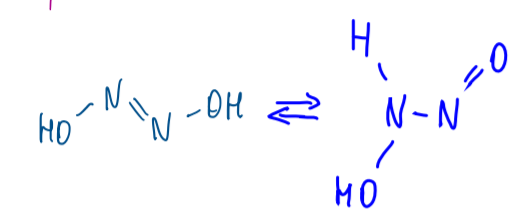
\includegraphics{images/8v12.png}

\subsubsection*{$HNO_2$-азотистая}

\textbf{Способы получения}

$$Ba(NO_2)_2 + H_2SO_4 \rightarrow BaSO_4\downarrow + HNO_2$$
$$N_2O_3 + H_2O \rightarrow HNO_3$$

\textbf{Химические свойства}

1) Разложение

$$HNO_2 \xrightarrow{>100^{\circ}} NO + HNO_3 + H_2O$$

2) ОВР

$$HNO_2 + Br_2 + H_2O \rightarrow HBr + HNO_3$$
$$HNO_2 + FeCl_2 + HCl \rightarrow FeCl_3 + NO + H_2O$$

\textbf{Строение}

Плоская молекула

\subsubsection*{$HNO_3$ - азотная кислота}

\textbf{Способы получения}

$$NH_3 + O_2 \xrightarrow{p,t,kat} NO + H_2O$$
$$NO + O_2 \rightarrow NO_2$$
$$NO_2+H_2O \rightarrow HNO_3 + HNO_2$$
$$HNO_3 \xrightarrow{t} NO + HNO_3 + H_2O$$

\textbf{Химические свойства}

1) Сильная кислота

2) Разложение при н.у (б/в)

$$HNO_3 \rightarrow NO_2 + O_2 + H_2O$$

3) Со многими металлами $H_2$ не выделяет, пассивирует $Fe,Cr,Al$

4) С неметаллами: $P, S, I,...$
$$ S + HNO_3 \rightarrow H_2SO_4 + NO_2 + H_2O$$

5) Нитраты растворимы в воде, при t разлагаются

$$KNO_3 \rightarrow KNO_2 + O_2$$
$$Cd(NO_3)_2 \rightarrow CdO + NO_2 + O_2$$
$$AgNO_3 \rightarrow Ag + NO_2 + O_2$$

6) Окислители в кислой среде и расплаве

$$MnO_2 + KOH + KNO_3 \rightarrow K_2MNO_4 + KNO_2 + H_2O$$

\textbf{Строение}

Плоская молекула

\subsubsection*{$NH_2OH$ - гидроксиламин}

\textbf{Способы получения}

$$6H^+ + HNO_3 + 6e^- \rightarrow NH_2OH + H_2O$$

\textbf{Химические свойства}

1) Разложение 

$$NH_2OH \rightarrow NH_3 + N_2 +H_2O$$

2) Основание 
$$NH_2OH \rightarrow H_2O \leftrightarrows NH_3OH^+ OH^-$$

3) Восстановитель (слабее $N_2H_4$)

$$NH_2OH + I_2 \rightarrow N_2 + HI + H_2O$$

4) Соль-окислитель

$$[NH_3OH]Cl + FeCl_2 + HCl \rightarrow NH_4Cl + FeCl_3 + H_2O$$

\textbf{Строение}

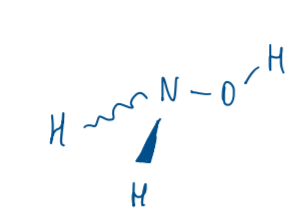
\includegraphics{images/8v13.png}

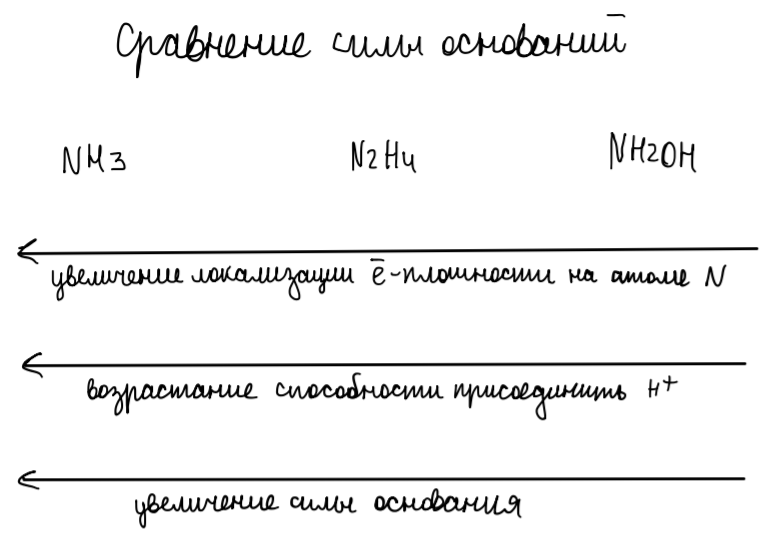
\includegraphics{images/8v14.png}
